\documentclass[]{elsarticle} %review=doublespace preprint=single 5p=2 column
%%% Begin My package additions %%%%%%%%%%%%%%%%%%%
\usepackage[hyphens]{url}

  \journal{Reproducible Research Workflow (GEO 712)} % Sets Journal name


\usepackage{lineno} % add
\providecommand{\tightlist}{%
  \setlength{\itemsep}{0pt}\setlength{\parskip}{0pt}}

\usepackage{graphicx}
\usepackage{booktabs} % book-quality tables
%%%%%%%%%%%%%%%% end my additions to header

\usepackage[T1]{fontenc}
\usepackage{lmodern}
\usepackage{amssymb,amsmath}
\usepackage{ifxetex,ifluatex}
\usepackage{fixltx2e} % provides \textsubscript
% use upquote if available, for straight quotes in verbatim environments
\IfFileExists{upquote.sty}{\usepackage{upquote}}{}
\ifnum 0\ifxetex 1\fi\ifluatex 1\fi=0 % if pdftex
  \usepackage[utf8]{inputenc}
\else % if luatex or xelatex
  \usepackage{fontspec}
  \ifxetex
    \usepackage{xltxtra,xunicode}
  \fi
  \defaultfontfeatures{Mapping=tex-text,Scale=MatchLowercase}
  \newcommand{\euro}{€}
\fi
% use microtype if available
\IfFileExists{microtype.sty}{\usepackage{microtype}}{}
\bibliographystyle{elsarticle-harv}
\usepackage{graphicx}
% We will generate all images so they have a width \maxwidth. This means
% that they will get their normal width if they fit onto the page, but
% are scaled down if they would overflow the margins.
\makeatletter
\def\maxwidth{\ifdim\Gin@nat@width>\linewidth\linewidth
\else\Gin@nat@width\fi}
\makeatother
\let\Oldincludegraphics\includegraphics
\renewcommand{\includegraphics}[1]{\Oldincludegraphics[width=\maxwidth]{#1}}
\ifxetex
  \usepackage[setpagesize=false, % page size defined by xetex
              unicode=false, % unicode breaks when used with xetex
              xetex]{hyperref}
\else
  \usepackage[unicode=true]{hyperref}
\fi
\hypersetup{breaklinks=true,
            bookmarks=true,
            pdfauthor={},
            pdftitle={Analysis and Modeling of Soil Respiration in a Turkey Point Deciduous Forest},
            colorlinks=false,
            urlcolor=blue,
            linkcolor=magenta,
            pdfborder={0 0 0}}
\urlstyle{same}  % don't use monospace font for urls

\setcounter{secnumdepth}{0}
% Pandoc toggle for numbering sections (defaults to be off)
\setcounter{secnumdepth}{0}
% Pandoc header
\usepackage{float}
\floatplacement{figure}{H}
\usepackage{pdflscape}
\newcommand{\blandscape}{\begin{landscape}}
\newcommand{\elandscape}{\end{landscape}}
\usepackage{booktabs}
\usepackage{longtable}
\usepackage{array}
\usepackage{multirow}
\usepackage{wrapfig}
\usepackage{float}
\usepackage{colortbl}
\usepackage{pdflscape}
\usepackage{tabu}
\usepackage{threeparttable}
\usepackage{threeparttablex}
\usepackage[normalem]{ulem}
\usepackage{makecell}
\usepackage{xcolor}



\begin{document}
\begin{frontmatter}

  \title{Analysis and Modeling of Soil Respiration in a Turkey Point Deciduous
Forest}
    \author[McMaster University School of Geography and Earth Sciences]{Yueqian (David) Ma}
   \ead{may118@mcmaster.ca} 
  
    \author[]{Katelynn M. Daly}
  
  
    \author[]{Myroslava Khomik}
   \ead{myroslava.khomik@hutton.ac.uk} 
  
    \author[]{Eric Beamesderfer}
   \ead{beamesde@mcmaster.ca} 
  
    \author[]{M. Altaf Arain}
   \ead{arainm@mcmaster.ca} 
  
      \address[McMaster University]{School of Geography and Earth Sciences, 1280 Main Street West, Hamilton,
Ontario, L8S 4L8}
  
  \begin{abstract}
  Soil water content and temperature are major controls on the soil carbon
  budget in forest ecosystems. Stored organic matter within the ecosystem
  is released into the atmosphere through heterotrophic and autotrophic
  activity referred to as soil respiration (Rs). An appropriate soil
  respiration model can assist in forest management and improve
  understanding of major environmental controls under future climate
  change. We collected and evaluated half-hourly data in the Global Water
  Futures (GWF) -- Southern Forests Water Future (SFWF)'s Turkey Point
  Deciduous Observatory from a closed-path eddy covariance system as well
  as automatic soil CO\textsubscript{2} efflux chambers (LI -- 8100A)
  which monitored Rs continuously since July 2014. Observed monthly mean
  Rs varied from a maximum of 7.50 µmol m\textsuperscript{-2}
  s\textsuperscript{-1} in July to a low of 1.11 µmol
  m\textsuperscript{-2} s\textsuperscript{-1} in December and showed a
  seasonal trend driven by soil temperature and water content. Three
  models: a general exponential regression model (Rs Ts),
  Q\textsubscript{10} with a logistic soil moisture function model (Rs
  SM), the Q\textsubscript{10} model (Rs Q\textsubscript{10}) were used to
  analyze Rs and soil temperature and soil water content controls.
  Comparison of the three models showed that the Rs SM model is best with
  an average yearly coefficient of determination of 0.68. The Rs SM model
  shows that by incorporating soil water content, it is able to improve
  upon models such as Q\textsubscript{10} that utilize soil temperature
  only to predict respiration. Study results show that Rs measurement and
  modeling studies should account for seasonal variations of temperature
  and water content within the soil. In addition, future work could
  include measurement of Rs during the winter and development of an
  accurate, predictive model.
  \end{abstract}
  
 \end{frontmatter}

\newlength{\cslhangindent}
\setlength{\cslhangindent}{1.5em}
\newenvironment{cslreferences}%
  {\setlength{\parindent}{0pt}%
  \everypar{\setlength{\hangindent}{\cslhangindent}}\ignorespaces}%
  {\par}

\hypertarget{introduction}{%
\section{1. Introduction}\label{introduction}}

Forests account for 3.7 billion hectares of the planet's surface area
and cover around 31\% of the world's land surface. They primarily
provide vital services at both global regional scales; including the
regulation of climate, hydrological cycles, air and water quality, and
biogeochemical cycles (Apps and Price, 1996; Matsumoto et al., 2008). In
addition to these ecosystem services, they provide significant economic
resources to various industries related to lumber, pulp, and
construction. \newline \newline Soil respiration (Rs) is the release of
CO\textsubscript{2} through heterotrophic and autotrophic activity and
accounts for 30 -- 80\% of net CO\textsubscript{2} release within
forests (Davidson and Janssens, 2006; Yiqi Luo and Xuhui Zhou, 2006).
Within the carbon cycle, 10\% of the atmospheric CO\textsubscript{2} is
passed through the soil each year primarily through organic matter decay
(Raich and Potter, 1995). Variability of Rs is influenced by diurnal,
seasonal, and annual patterns along with multiple factors such as soil
moisture and temperature. When compared to the atmosphere and biotic
sinks the soil carbon sink is 3.2 and 4 times larger, respectively
(Edenhofer, 2014; Lorenz and Lal, 2010). On account of the storage
differences, a small change in Rs due to improper management techniques
can result in a large release of CO\textsubscript{2} into the
atmosphere. \newline \newline Quantifying Rs can indicate various
physiological processes, as well as the ability of soil to support life
including plants, animals, and microorganisms (L. Liu et al., 2016). By
modeling, mapping, and monitoring flux movement, forest management
techniques can be utilized to decrease the amount of CO\textsubscript{2}
released into the atmosphere. Changes in Rs rates can also indicate
external processes, such as disturbance (for example cultivation) which
typically increases Rs (Schlesinger and Andrews, 2000). \newline
\newline Rs models can be classified into two types: empirical and
mechanistic. Empirical models typically use regressional analysis of Rs
with temperature and moisture which is derived from observed data.
Mechanistic models are created using environmental and biological
factors that contribute to Rs. These models can be categorized into two
parts: the CO\textsubscript{2} production model; which considers factors
that produce CO\textsubscript{2}, and the CO\textsubscript{2}
production-transport models; which considers CO\textsubscript{2}
production along with its transport to the soil surface. \newline
\newline The specific objectives of this study are to (1) gain a better
understanding of the spatial and temporal dynamics of Rs, (2) determine
how Rs responds to its main controlling variables (i.e.~soil temperature
and soil moisture), (3) help determine the impact of extreme weather
events on Rs, (4) to compare several different models with varying
complexity using a wide range of parameters, and (5) to determine which
model produces the best fit and Rs estimation.

\hypertarget{materials-and-methods}{%
\section{2. Materials and Methods}\label{materials-and-methods}}

This study was conducted in a 90 -- year old managed deciduous
(Carolinian species) forest (TPD) northwest of Long Point Provincial
Park in Southern Ontario, Canada (42.64\textsuperscript{o}N,
80.56\textsuperscript{o}W). The forest is naturally regenerated on sandy
terrain and abandoned agricultural land, and has been managed (thinned
in the past). Predominant tree species include: white oak
(\textit{Quercus alba}), sugar and red maple
(\textit{Acer saccharum, A. rubrum}), american beech
(\textit{Facus grandifolia}), black and red oak
(\textit{Q. veluntia, Q. rubra}), and white ash
(\textit{Fraxinus americana}). Average tree height is 25.7 m with a
diameter at breast height of 22.3 cm. The leaf area index (LAI) of the
site was measured by a canopy analyzer (model LAI-2000, LI-COR, Lincoln,
Nebraska, USA) and TRAC (Tracing Radiation and Architecture of Canopy,
developed by Dr.~Jin M. Chen's group at the University of Toronto). This
site is part of the Turkey Point Flux Station (TPFS) and associated with
Ameriflux and global Fluxnet Networks. Further site information is found
in Table \ref{tab:site_description}. \newline \newline The topography is
undulating, with well -- drained, mostly sandy soil (Brunisolic Gray
Brown Luvisol) with low to moderate water holding capacity. The soil
organic layer depth typically ranged from 2 to 6 cm. In September of
2014, soil cores and litter samples were taken and sent for nutrient
analysis (A \& L Canada Laboratories, Inc., London, Ontario). The
samples were analyzed for total organic matter content, carbon,
nitrogen, phosphorus, potassium, magnesium, calcium, and other
additional soil characteristics. The soil nutrient content is outlined
in Table \ref{tab:topography}. 30 -- year climate normal, based on 1981
-- 2010 Environment Canada weather data collected at Delhi, Ontario CDA
weather station, indicate a mean annual temperature of
8.0\textsuperscript{o}C and mean annual precipitation (PPT) of 136 mm
(906.4 mm of which falls as rain and 129.5 cm as snow). \newline
\newline Continuous Rs was recorded using an automated soil
CO\textsubscript{2} flux measurement system, taking half hourly
measurements from July 2014 to November 2018 for the snow free growing
season. Measurements are comprised of 3 main components: the gas
analyzer (hosted in an analyzer control unit) (LI-8100A), long term
measurement chambers (LI8100 -- 104), and a multiplexer to allow for
multiple chamber measurements (LI-8150) (LI-COR Lincoln, Nebraska, USA.
Two measurement chambers were deployed from July to December 2014, and
increased to five in April 2015. Each chamber extended approximately 15
m from the central analyzer control unit and multiplexer, measuring half
-- hourly Rs in sequence. Chambers are equipped with a soil temperature
(Ts) and soil moisture (SM) probe (LI8150 -- 203 and LI8150 -- 205
respectively) at 5 cm depth installed outside of the collar. \newline
\newline The soil collars are comprised of thick -- walled PVC pipe with
an internal diameter of approximately 20 cm, a height of 11.5 cm, and a
thickness of 1 cm. Each collar is inserted approximately 7 -- 8 cm into
the soil surface, with 3 cm remaining above. The measurement chamber is
placed directly on the soil collar, remaining open when not taking
active measurements. Throughout the growing season, any vegetation
growth as removed from inside the collars to eliminate potential
photosynthesis effects. \newline \newline Measurements from the first
chamber was removed from 2014 to 2017 due to a wasp nest causing
increased CO\textsubscript{2} reports. Data is processed using Soil Flux
Pro (4.0.1) from LI-COR Biosciences, Inc.~by analyzing the exponential
flux and iteration obtained every 3 -- 4 min within the 30 min
measurement period. The exponential flux is the CO\textsubscript{2} flux
determined by the exponential fit which uses the dilution corrected
CO\textsubscript{2} (C) plotted against time in seconds (the difference
between the start and stop time) (t) (Equation 1). The resulting plot is
fit with a non-linear regression equation that solves for
C\textsubscript{\(\infty\)}, t\textsubscript{0}, and \(\alpha\) where
C\textsubscript{o} is the starting measured CO\textsubscript{2}
concentration. The CO\textsubscript{2} flux based on the slope of the
regression equation is reported as the exponential flux.

\[ C(t) = C_\infty + (C_0 - C\infty)e^{-\alpha(t-t_0)} \]

Measurements that report a higher exponential iteration (greater than
10) was processed further by changing the start time affecting the
overall t value until the exponential iteration is less than 10.
\newline \newline Linear and non-linear analyses are performed on daily
measure of measured Rs data for gap filling. Three models are derived to
determine the correlation between Rs and its environmental controls,
outlined in Table \ref {tab:models}. The first is a simple, exponential
regression between Rs and Ts (Rs Ts) by Hoff and Lehfeldt (1899), the
second is the annual temperature response model (Rs
Q\textsubscript{10}). The third is the Q\textsubscript{10} model
modified with a logistic function (Khomik et al., 2010) to incorporate
soil moisture effects (Rs SM). The models are evaluated using 70\% of
observed measurements for training and 30\% of data for model testing.
\newline \newline Each model was used to simulate daily, yearly, and
seasonal (spring = March -- May, summer = June -- August, Autumn =
September -- November, Winter = December -- February) and growing season
(March -- November) Rs emissions, and compared to ecosystem respiration
(RE) data derived from eddy covariance measurements. The models are
evaluated using coefficient of determination (R2), error sum of squares
(SSE), standard deviation (STD), relative error (RE), slope and
intercept of the testing function to Y = x, and yearly fit to observed
Rs. \newline \newline The daily Rs recorded by automated chamber
measurements during the study period are shown in Figure
\ref{fig:rstimeSeries}. The seasonal trend of Rs follow closely that of
Ta and Ts, reaching maximum values in the summer months, then followed a
declining trend throughout the rest of the year. An increase in Rs
during and following precipitation events was observed. For example, on
September 2nd, 2014 there was a 22.4 mm precipitation event which caused
an increase of SM from 0.1 to 0.28 m\textsuperscript{3}
m\textsuperscript{-3} and an 88\% increase from 6.5 to 12.2 µmol
CO\textsubscript{2} m\textsuperscript{-2} s\textsuperscript{-1} (Figure
\ref{fig:rainEvent2014}). \newline \newline Rs did not return of
pre-rain event Rs until September 8th, 6 days after the rain event. On
October 9th, 2017 there was a 11.7 mm precipitation event which caused
an SM increase of 0.1 to 0.39 m3m-3 and an 78\% in Rs from 5.97 to 10.63
µmol CO\textsubscript{2} m\textsuperscript{-2} s\textsuperscript{-1}
(Figure \ref{fig:rainEvent2017}) until October 29, 20 days after the
rain event. Rs coverage at the site is 36.71\%, 55.07\%, 55.07\%,
50.68\%, and 55.62\% from 2014 to 2018.

\hypertarget{results}{%
\section{3. Results}\label{results}}

A comparison of modeled and observed daily mean Rs during the growing
season for all years are shown in (Figure \ref{fig:rsEstTest}). The
modeled vs observed regression analysis and the coefficient of
determination of each model is shown in Table \ref {tab:modelTrain}.
Model relative error is shown in (Figure \ref{fig:barOut}) and standard
deviation with error sum of squares are shown in Table
\ref {tab:rsStats}. In all years (with the exception of 2014 and 2016)
the Rs SM model produced the highest correlation coefficient and the
lowest SSE. The relative error between the Rs Ts and Rs
Q\textsubscript{10} is relatively similar with a standard deviation
\newline \newline To better visualize the temporal trends in model fit,
the daily relative error of each fitted models is plotted in a stacked
bar plot over the study period (Figure \ref{fig:barOut}). There were
clear seasonal trends for all of the models. In all of the years, the
models produced a positive relative error values during the summer
months (June, July, and August), representing an underestimation of Rs
values. Towards April/May to the summer months and at the end of August
towards the end of the measurement period, the models were produced
negative relative error indicating an overestimation of Rs. There were
large relative error values at the end of 2014 and at the beginning of
2016 to 2018 which could be the result of instrumentation problems
resulting in a loss of Rs data, inhibiting the ability to produce a
model that accurately predicts Rs during that season. Another
possibility could be due to high temperatures in 2016 which is followed
by a high precipitation event in 2017 and the re-addition of another
chamber in 2018. \newline \newline When daily relative error is plotted
against a function of temperature, (Figure \ref{fig:tempRE}) Rs Ts and
Rs Q\textsubscript{10} is shown to have similar relative error values
with all models resulting in positive relative errors during high
temperatures and negative relative errors at low temperatures (with the
exception of 2017 and 2018). In 2017, relative error was uniform at
higher temperatures indicating better model prediction. In 2018,
relative error was consistent throughout temperature ranges due to the
addition of another chamber and increased training sample size. \newline
\newline Each model was used to simulate seasonal and growing seasonal
Rs emissions which are summarized in Table \ref {tab:seasons}. Across
the three models, spring had the lowest carbon emissions. The highest
estimates were in the summer season, with emissions declining again the
autumn and winter. No model estimated below 1200 m\textsuperscript{-2}
s\textsuperscript{-1} in 2014, 2017 and 2018.

\hypertarget{discussion-and-conclusion}{%
\section{4. Discussion and Conclusion}\label{discussion-and-conclusion}}

The effect of temperature on Rs can be expressed using the
Q\textsubscript{10} model coefficients, R\textsubscript{10} and
Q\textsubscript{10} (Table \ref {tab:modelTrain}. The basal respiration
rate at 10\textsuperscript{o}C (R\textsubscript{10}) is related to the
volume of the soil column that is biologically active, i.e.~the size and
activity of microbial and root population (Mo et al., 2005).The
Q\textsubscript{10} value is the temperature sensitivity of Rs to
warming (Jia et al. (2013)). The Q\textsubscript{10} values obtained at
our site were found to range from 1.70 to 2.36 (Table
\ref {tab:modelTrain}) and R\textsubscript{10} values ranged from 2.84
to 4.73. This was found to be within range of literature -- reported
values (Greco and Baldocchi, 1996; Tang et al., 2014; Xu et al., 2004)
and followed distinct seasonal trends. \newline \newline Few studies
have quantified the total contributions of Rs pulses following rain
events to total Rs. Lee et al. (2002) reported an increase in Rs rates
of 16 -- 21\% following rain events in a temperate deciduous forest in
Japan. B. Liu et al. (2016) conducted a meta -- analysis on
precipitation treatments across multiple biomes and found that
precipitation events in temperate forests cause an increase in Rs of 17
-- 30\%. Furthermore, drought can also influence soil respiration. The
study concluded that longer drought periods showed an increase in soil
and heterotrophic respiration in accordance to the period of drought.
This is shown in (\ref{fig:droughtEvent}) where after a long period of
drought in September 2017 (a period of 19 days; Figure
\ref {fig:smPPT}), a precipitation event caused a spike in Rs greater
than those seen in early to mid -- summer. \newline \newline 2014 models
produced a poor yearly fit and coefficient of determination mainly
because of 3 factors: the lack of data coverage from measurement later
within the season, the removal of one chamber due to high
CO\textsubscript{2} measurement from a wasp nest, and the number of
chambers (3 in 2014 compared to 5 in 2015). This resulted in dependent
on time series data training to produce a worse fit. More complex models
(Rs SM) produced a spike in Rs during the measurement period and low Rs
before the period. Whereas models such as Rs Ts and Rs
Q\textsubscript{10} produced a constant increase and decrease throughout
the year. This is likely due to seasonal bias causing the equations to
underestimate indicating that in years with no extreme events or
anomalies, a simpler model is suitable for estimation. \newline \newline
2015 models on average produced a higher coefficient of determination
with the addition of more chambers. However, the Rs Q\textsubscript{10}
and Rs Ts model produced a much lower increase indicating that the
annual Q\textsubscript{10} model may not reflect true temperature
sensitivity since it can be obscured by other seasonally -- varying
factors such as root biomass, photosynthesis rates, and litter inputs
(Curiel yuste et al., 2004; Gaumont-Guay et al., 2006). When
incorporating soil moisture, the models produced a better yearly fit.
Soil moisture has numerous effects on ecosystem metabolism and growth,
and thus is an important factor influencing low Rs. Low soil moisture
conditions can decrease the temperature sensitivity and lower the
overall rate of Rs (Davidson and Janssens, 2006; van der Molen et al.,
2011; Xu and Qi, 2001). High soil moisture can limit the diffusion of
oxygen to microbial communities for relative humidity (Pumpanen et al.,
2008). \newline \newline 2016 models produced an average low fit because
of low precipitation and higher yearly temperatures creating relatively
low Rs compared to previous years causing models dependent on soil
temperature and moisture to underestimate. 2017 models produced a
slightly better fit compared to 2016, however because of an extremely
high precipitation event, the overall fit is comparably less than 2014
and 2015. All models have a close relationship with Ts and follows the
Ts curve accordingly each year. However, because of the high amount of
Ts early within the season due to a high precipitation event (57.39 mm),
the models based on only Ts overestimated Rs early within the growing
season (Rs Ts, Rs Q\textsubscript{10}). \newline \newline This event was
closely followed with another, slightly lower precipitation event (39.70
mm) which caused Rs to rapidly increase and models to underestimate. In
October 9th, there was an extreme precipitation event of 81.44 mm
causing Rs to spike to 11.86 µmol CO\textsubscript{2}
m\textsuperscript{-2} s\textsuperscript{-1}. However, because the soil
moisture did not increase as high due to excess saturation of the ground
and runoff, models dependent on both soil temperature and soil moisture
underestimated Rs (Rs SM). \newline \newline 2018 models are able to
produce a better yearly fit because of a one measurement chamber being
re-introduced increasing the amount of training data. The year showed
relatively similar soil temperature and moisture to 2014 and 2015 with
no extreme precipitation events. There were two spikes in Rs in July and
September corresponding to two precipitation events the first of which
(July) caused underestimation in models using only Ts and SM. The second
spike in Rs (September) was able to be accurately predicted by all
models involving soil moisture. \newline \newline This study has
provided important insight on the temporal and spatial dynamics of Rs.
The addition of temporal and SM considerations have shown to increase
the modeling accuracy of traditional models such as Q\textsubscript{10}.
Many future climate change scenarios predict an increased probability of
intense precipitation events (Edenhofer, 2014), and a quantitative
understanding of the Rs rain response is a necessary consideration in
the development of an accurate global carbon cycle model. Future work
could include a quantification of the contribution of precipitation --
induced pulses in Rs to annual total Rs in temperate deciduous forests,
considering the measurement of Rs during the winter, as well as the
further development of an accurate, predictive model through improved
understanding of spatial and temporal dynamics of Rs.

\pagebreak

\hypertarget{tables-and-figures}{%
\section{Tables and Figures}\label{tables-and-figures}}

\begin{table}[!h]

\caption{\label{tab:site_info-1}\label{tab:site_description} Site description of a 90 - year old managed deciduous (Carolian species) forest.}
\centering
\fontsize{8}{10}\selectfont
\begin{tabular}[t]{ll}
\toprule
Characteristic & Description\\
\midrule
\rowcolor{gray!6}  Water Table Depth (m) & 2 - 3.5\\
Stand Density (Trees $Ha^-$$^1$) & 504±5\\
\rowcolor{gray!6}  Area (Ha) & 49\\
LAI ($m^2 m^-$$^2$) & 8.00\\
\rowcolor{gray!6}  Elevation (m) & 210.60\\
\addlinespace
Climate & Cool, temperate\\
\rowcolor{gray!6}  Mean Temperature ($^o$C) & 7.80\\
Precipitation (mm) & 1010\\
\rowcolor{gray!6}  soil pH & 5.00\\
\bottomrule
\end{tabular}
\end{table}

\begin{table}[!h]

\caption{\label{tab:site_info-2}\label{tab:topography} Selected values of soil nutrient content of litter fall horizon (LFH), Turkey Point Deciduous (TPD).}
\centering
\resizebox{\linewidth}{!}{
\begin{tabular}[t]{llllllll}
\toprule
Soil Layer & OM (\%) & P (ppm) & K (ppm) & Mg (ppm) & Ca (ppm) & pH & C/N Ratio\\
\midrule
\rowcolor{gray!6}  Litter & 28.80 & 93.00 & 127.00 & 274.30 & 2186.00 & 6.00 & 15.90\\
0 to 15 cm & 3.50 & 126.00 & 24.00 & 52.00 & 458.00 & 4.90 & 13.30\\
\rowcolor{gray!6}  15 to 35 cm & 1.30 & 170.00 & 10.00 & 33.00 & 315.00 & 5.30 & 12.70\\
\bottomrule
\end{tabular}}
\end{table}

\begin{table}[!h]

\caption{\label{tab:site_info-3}\label{tab:models} Selected values of soil nutrient content of litter fall horizon (LFH), Turkey Point Deciduous (TPD).}
\centering
\resizebox{\linewidth}{!}{
\begin{tabular}[t]{lll}
\toprule
Model & Formula & References\\
\midrule
\rowcolor{gray!6}  Rs Ts & Rs = ae$^b$$^T$$^s$ & Hoff and Lehfeldt (1899)\\
Rs $Q_1$$_0$ & Rs = $R_1$$_0$$Q_1$$_0$ $^($$^T$$^s$$^-$$^1$$^0$$^)$$^/$$^1$$^0$ & Curiel Yuste et al. (2004)\\
\rowcolor{gray!6}  Rs SM & Rs SM = $R_1$$_0$$Q_1$$_0$ $^($$^T$$^s$$^-$$^1$$^0$$^)$$^/$$^1$$^0$ * (1/1+e$^a$$^+$$^b$$^*$$^S$$^M$) & Chan et al. (2018)\\
\bottomrule
\end{tabular}}
\end{table}

\begin{table}[!h]

\caption{\label{tab:site_info-4}\label{tab:modelTrain} Training results and coefficient of determination ($R^2$) for the Rs Ts, Rs Q$_1$$_0$, Rs SM models from 2014 to 2018.}
\centering
\fontsize{8}{10}\selectfont
\begin{tabular}[t]{cccccccc}
\toprule
Models & Variables & 2014 & 2015 & 2016 & 2017 & 2018 & All\\
\midrule
\rowcolor{gray!6}  Rs Ts & a & 2.29 & 1.79 & 1.67 & 2.61 & 1.49 & 2.25\\
 & b & 0.072 & 0.056 & 0.053 & 0.052 & 0.085 & 0.054\\
\rowcolor{gray!6}   & R$^2$ & 0.71 & 0.54 & 0.44 & 0.48 & 0.74 & 0.38\\
 &  &  &  &  &  &  \vphantom{1} & \\
\rowcolor{gray!6}  Rs Q$_1$$_0$ & R$_1$$_0$ & 7.43 & 3.14 & 2.84 & 4.36 & 3.51 & 3.87\\
\addlinespace
 & Q$_1$$_0$ & 2.06 & 1.76 & 1.70 & 1.67 & 2.36 & 1.72\\
\rowcolor{gray!6}   & R$^2$ & 0.71 & 0.54 & 0.44 & 0.48 & 0.75 & 0.38\\
 &  &  &  &  &  &  & \\
\rowcolor{gray!6}  Rs SM & R$_1$$_0$ & 6.07 & 3.87 & 2.77 & 4.30 & 3.97 & 4.12\\
 & Q$_1$$_0$ & 2.51 & 2.32 & 2.03 & 1.89 & 2.76 & 2.14\\
\addlinespace
\rowcolor{gray!6}   & a & 1.17 & 0.89 & 1.46 & 0.90 & 0.029 & 0.49\\
 & b & -17.67 & -17.55 & -87.91 & -63.23 & -18.65 & -26.90\\
\rowcolor{gray!6}   & R$^2$ & 0.82 & 0.76 & 0.54 & 0.64 & 0.85 & 0.52\\
\bottomrule
\end{tabular}
\end{table}

\begin{table}[!h]

\caption{\label{tab:site_info-5}\label{tab:rsStats} Statistics for applied Rs models; error sum of squares (SSE) and standard deviation (STD).}
\centering
\fontsize{8}{10}\selectfont
\begin{tabular}[t]{lllllll}
\toprule
\multicolumn{1}{c}{Year} & \multicolumn{2}{c}{Rs Ts} & \multicolumn{2}{c}{Rs Q$_1$$_0$} & \multicolumn{2}{c}{Rs SM} \\
\cmidrule(l{3pt}r{3pt}){1-1} \cmidrule(l{3pt}r{3pt}){2-3} \cmidrule(l{3pt}r{3pt}){4-5} \cmidrule(l{3pt}r{3pt}){6-7}
\rowcolor{gray!6}   & SSE & STD & SSE & STD & SSE & STD\\
2014 & 86.86 & 2.49 & 86.91 & 2.50 & 111.20 & 2.63\\
\rowcolor{gray!6}  2015 & 72.15 & 1.26 & 72.23 & 1.25 & 54.52 & 1.63\\
2016 & 41.32 & 1.10 & 41.35 & 1.10 & 42.16 & 1.24\\
\rowcolor{gray!6}  2017 & 57.18 & 1.56 & 57.08 & 1.55 & 56.83 & 1.68\\
\addlinespace
2018 & 233.60 & 2.63 & 233.40 & 2.63 & 152.70 & 2.73\\
\bottomrule
\end{tabular}
\end{table}

\begin{table}[!h]

\caption{\label{tab:site_info-6}\label{tab:seasons} Estimated seasonal and total Rs over the growing season from 2014 to 2018.}
\centering
\resizebox{\linewidth}{!}{
\begin{tabular}[t]{llllllllllllllll}
\toprule
\multicolumn{1}{c}{Season} & \multicolumn{3}{c}{2014(in thousands)} & \multicolumn{3}{c}{2015
(in thousands)} & \multicolumn{3}{c}{2016
(in thousands)} & \multicolumn{3}{c}{2017
(in thousands)} & \multicolumn{3}{c}{2018
(in thousands)} \\
\cmidrule(l{3pt}r{3pt}){1-1} \cmidrule(l{3pt}r{3pt}){2-4} \cmidrule(l{3pt}r{3pt}){5-7} \cmidrule(l{3pt}r{3pt}){8-10} \cmidrule(l{3pt}r{3pt}){11-13} \cmidrule(l{3pt}r{3pt}){14-16}
\rowcolor{gray!6}  Model & RsTs & Rs$Q_1$$_0$ & RsSM & RsTs & Rs$Q_1$$_0$ & RsSM & RsTs & Rs$Q_1$$_0$ & RsSM & RsTs & Rs$Q_1$$_0$ & RsSM & RsTs & Rs$Q_1$$_0$ & RsSM\\
Spring & 3.33 & 3.33 & 3.16 & 2.40 & 2.40 & 2.14 & 2.32 & 2.32 & 2.14 & 3.61 & 3.61 & 3.50 & 2.53 & 2.53 & 2.57\\
\rowcolor{gray!6}  Summer & 7.49 & 7.49 & 6.47 & 4.43 & 4.43 & 4.77 & 4.13 & 4.13 & 4.77 & 6.00 & 6.00 & 5.92 & 6.80 & 6.80 & 6.43\\
Autumn & 4.99 & 4.99 & 4.98 & 3.42 & 3.42 & 2.92 & 3.22 & 3.13 & 2.92 & 4.64 & 4.64 & 4.38 & 4.34 & 4.34 & 4.56\\
\rowcolor{gray!6}  Winter & 2.34 & 2.24 & 1.67 & 1.62 & 1.62 & 1.08 & 1.28 & 1.28 & 1.08 & 2.59 & 2.59 & 2.31 & 1.52 & 1.52 & 1.38\\
\addlinespace
Total & 18.05 & 18.05 & 16.27 & 11.86 & 11.87 & 10.92 & 10.86 & 10.86 & 10.84 & 16.85 & 16.85 & 16.11 & 15.19 & 15.19 & 14.93\\
\bottomrule
\end{tabular}}
\end{table}
\clearpage

\begin{figure}
\centering
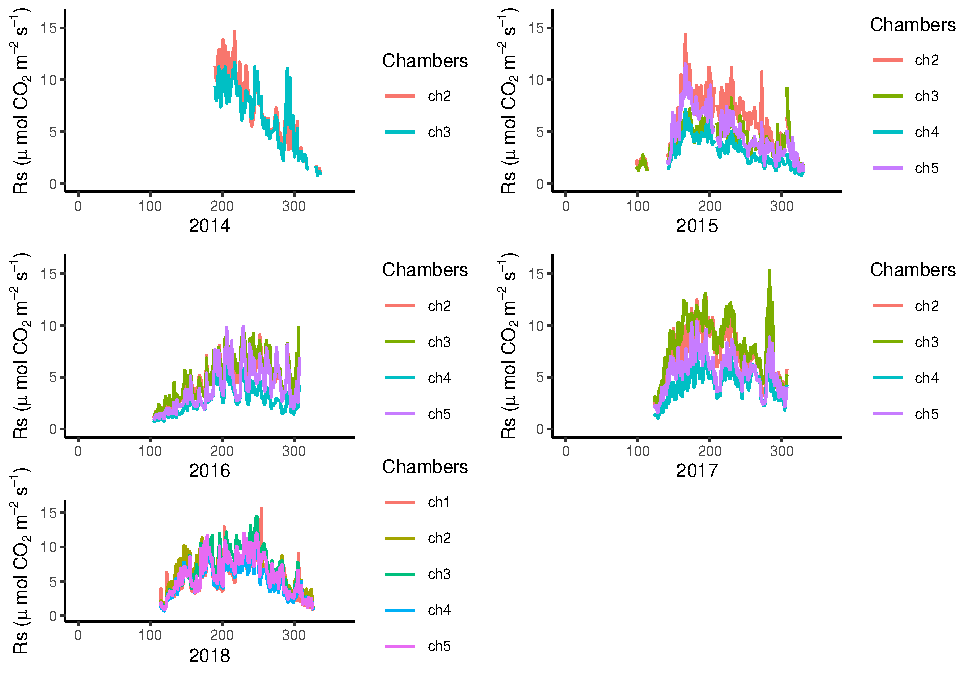
\includegraphics{TPD_Paper_files/figure-latex/timeSeries-1.pdf}
\caption{\label{fig:rstimeSeries} Daily average soil respiration (Rs) in
µmol CO\(_2\) m\(^-\)\(^2\) s\(^-\)\(^1\) measured by automated soil
CO\(_2\) chamber systems over a 5 year study period}
\end{figure}

\begin{figure}
\centering
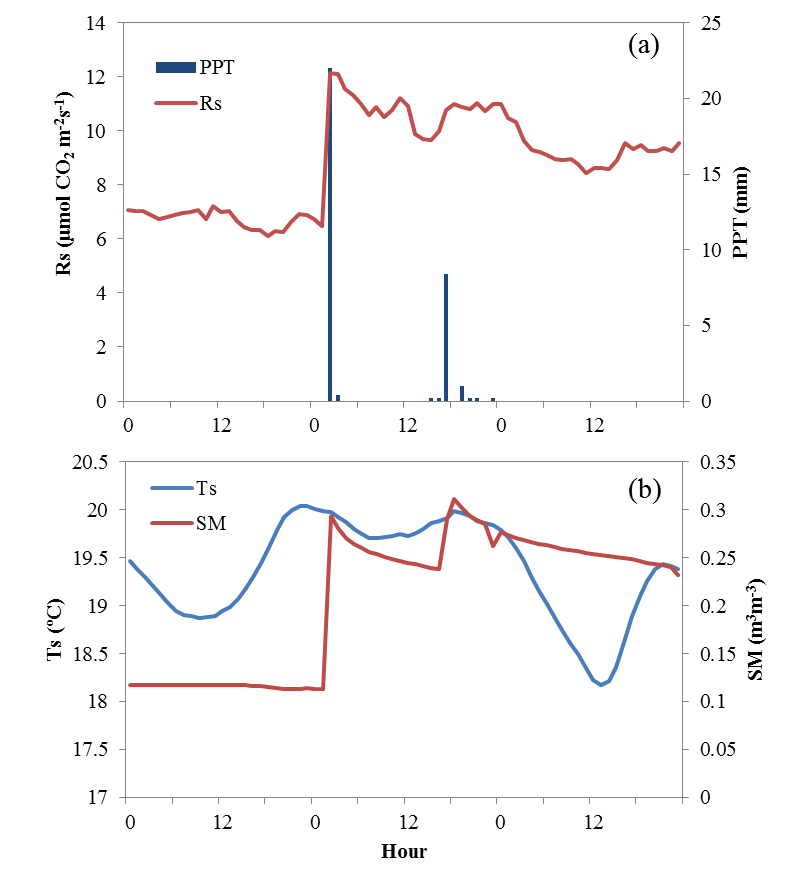
\includegraphics{../images/static/rainEvent2014.png}
\caption{(a) Half hourly soil respiration (Rs) and precipitation (PPT)
and (b) half hourly soil temperature (Ts) and soil moisture (SM) at 5
cmd depth before, during, and after following a 22.4 mm precipitation
event on September 2, 2014 \label{fig:rainEvent2014}}
\end{figure}

\begin{figure}
\centering
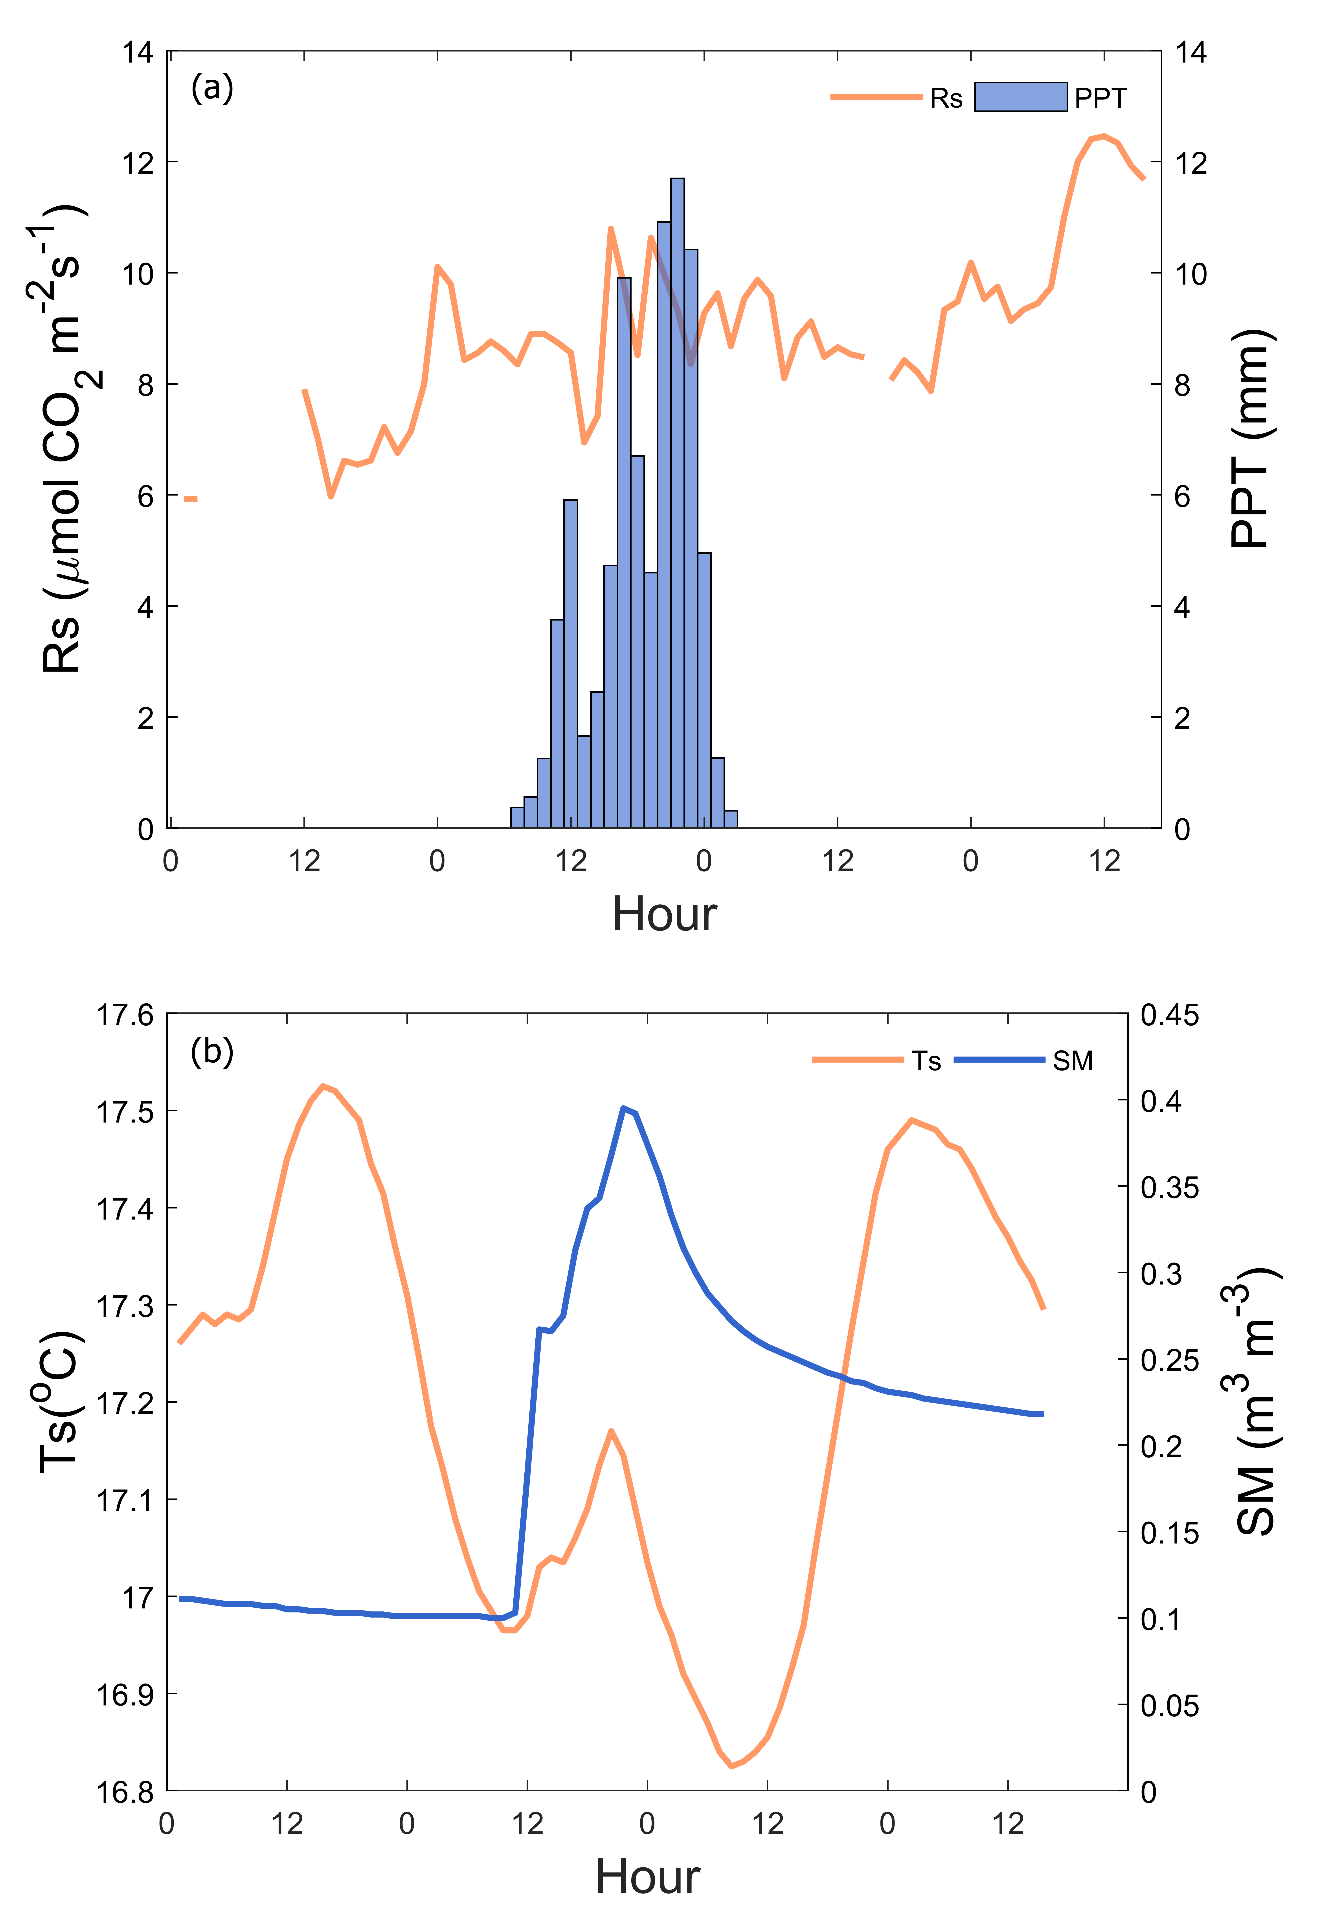
\includegraphics{../images/static/rainEvent2017.png}
\caption{(a) Half hourly soil respiration (Rs) and precipitation (PPT)
and (b) half hourly soil temperature (Ts) and soil moisture (SM) at 5 cm
depth before, during, and after following a 11.7 mm precipitation on
October 7, 2017 \label{fig:rainEvent2017}}
\end{figure}

\begin{figure}
\centering
\includegraphics{../images/static/allModels.png}
\caption{Annual observed Rs values compared with predicted values using
three models (Rs Ts, Rs Q\(_1\)\(_0\) Rs SM) from 2014 to 2018 recoreded
in µmol CO\(^2\) m\(^-\)\(^2\) s\(^-\)\(^1\) \label{fig:rsEstTest}}
\end{figure}

\begin{figure}
\centering
\includegraphics{../images/static/RE_Ts_3mod.png}
\caption{The daily relative error of Rs Ts, Rs Q\(_1\)\(_0\), and Rs SM
plotted against temperature (\(^o\)C) for the growing season from 2014
to 2018. \label{fig:tempRE}}
\end{figure}

\clearpage
\begin{landscape}

\begin{figure}
\centering
\includegraphics{../images/static/barOut.png}
\caption{Stacked bar plot showing the daily relative error of Rs Ts, Rs
Q\(_1\)\(_0\), Rs SM models over the 2014 to 2018 measurement period
\label{fig:barOut}}
\end{figure}

\begin{figure}
\centering
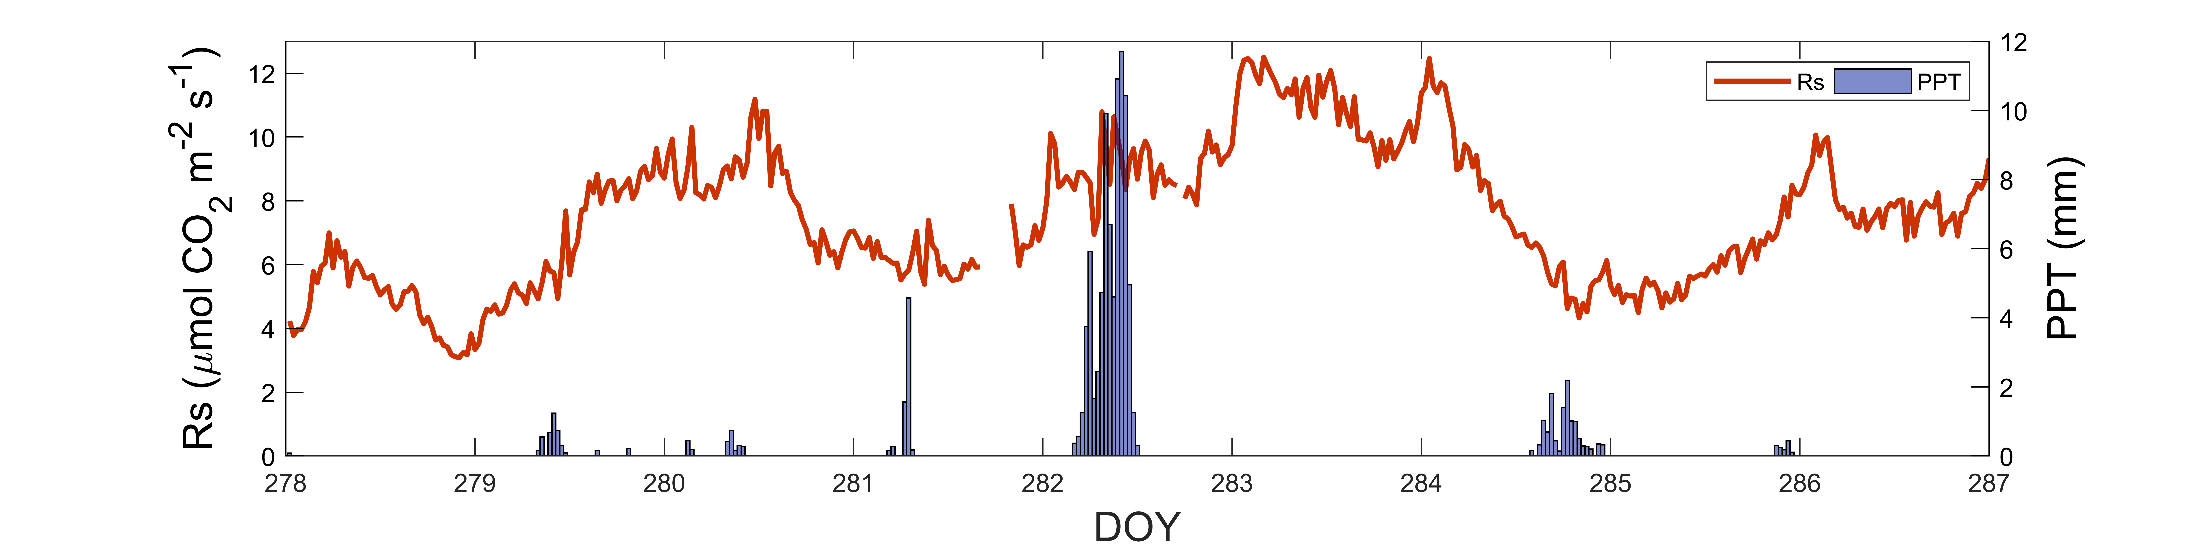
\includegraphics{../images/static/droughtEvent.png}
\caption{Precipitation event (mm) and Rs (µmol CO\(^2\) m\(^-\)\(^2\)
s\(^-\)\(^1\)) from October 5 to 13 in 2017 following a drought of 19
days \label{fig:droughtEvent}}
\end{figure}

\end{landscape}

\begin{figure}
\centering
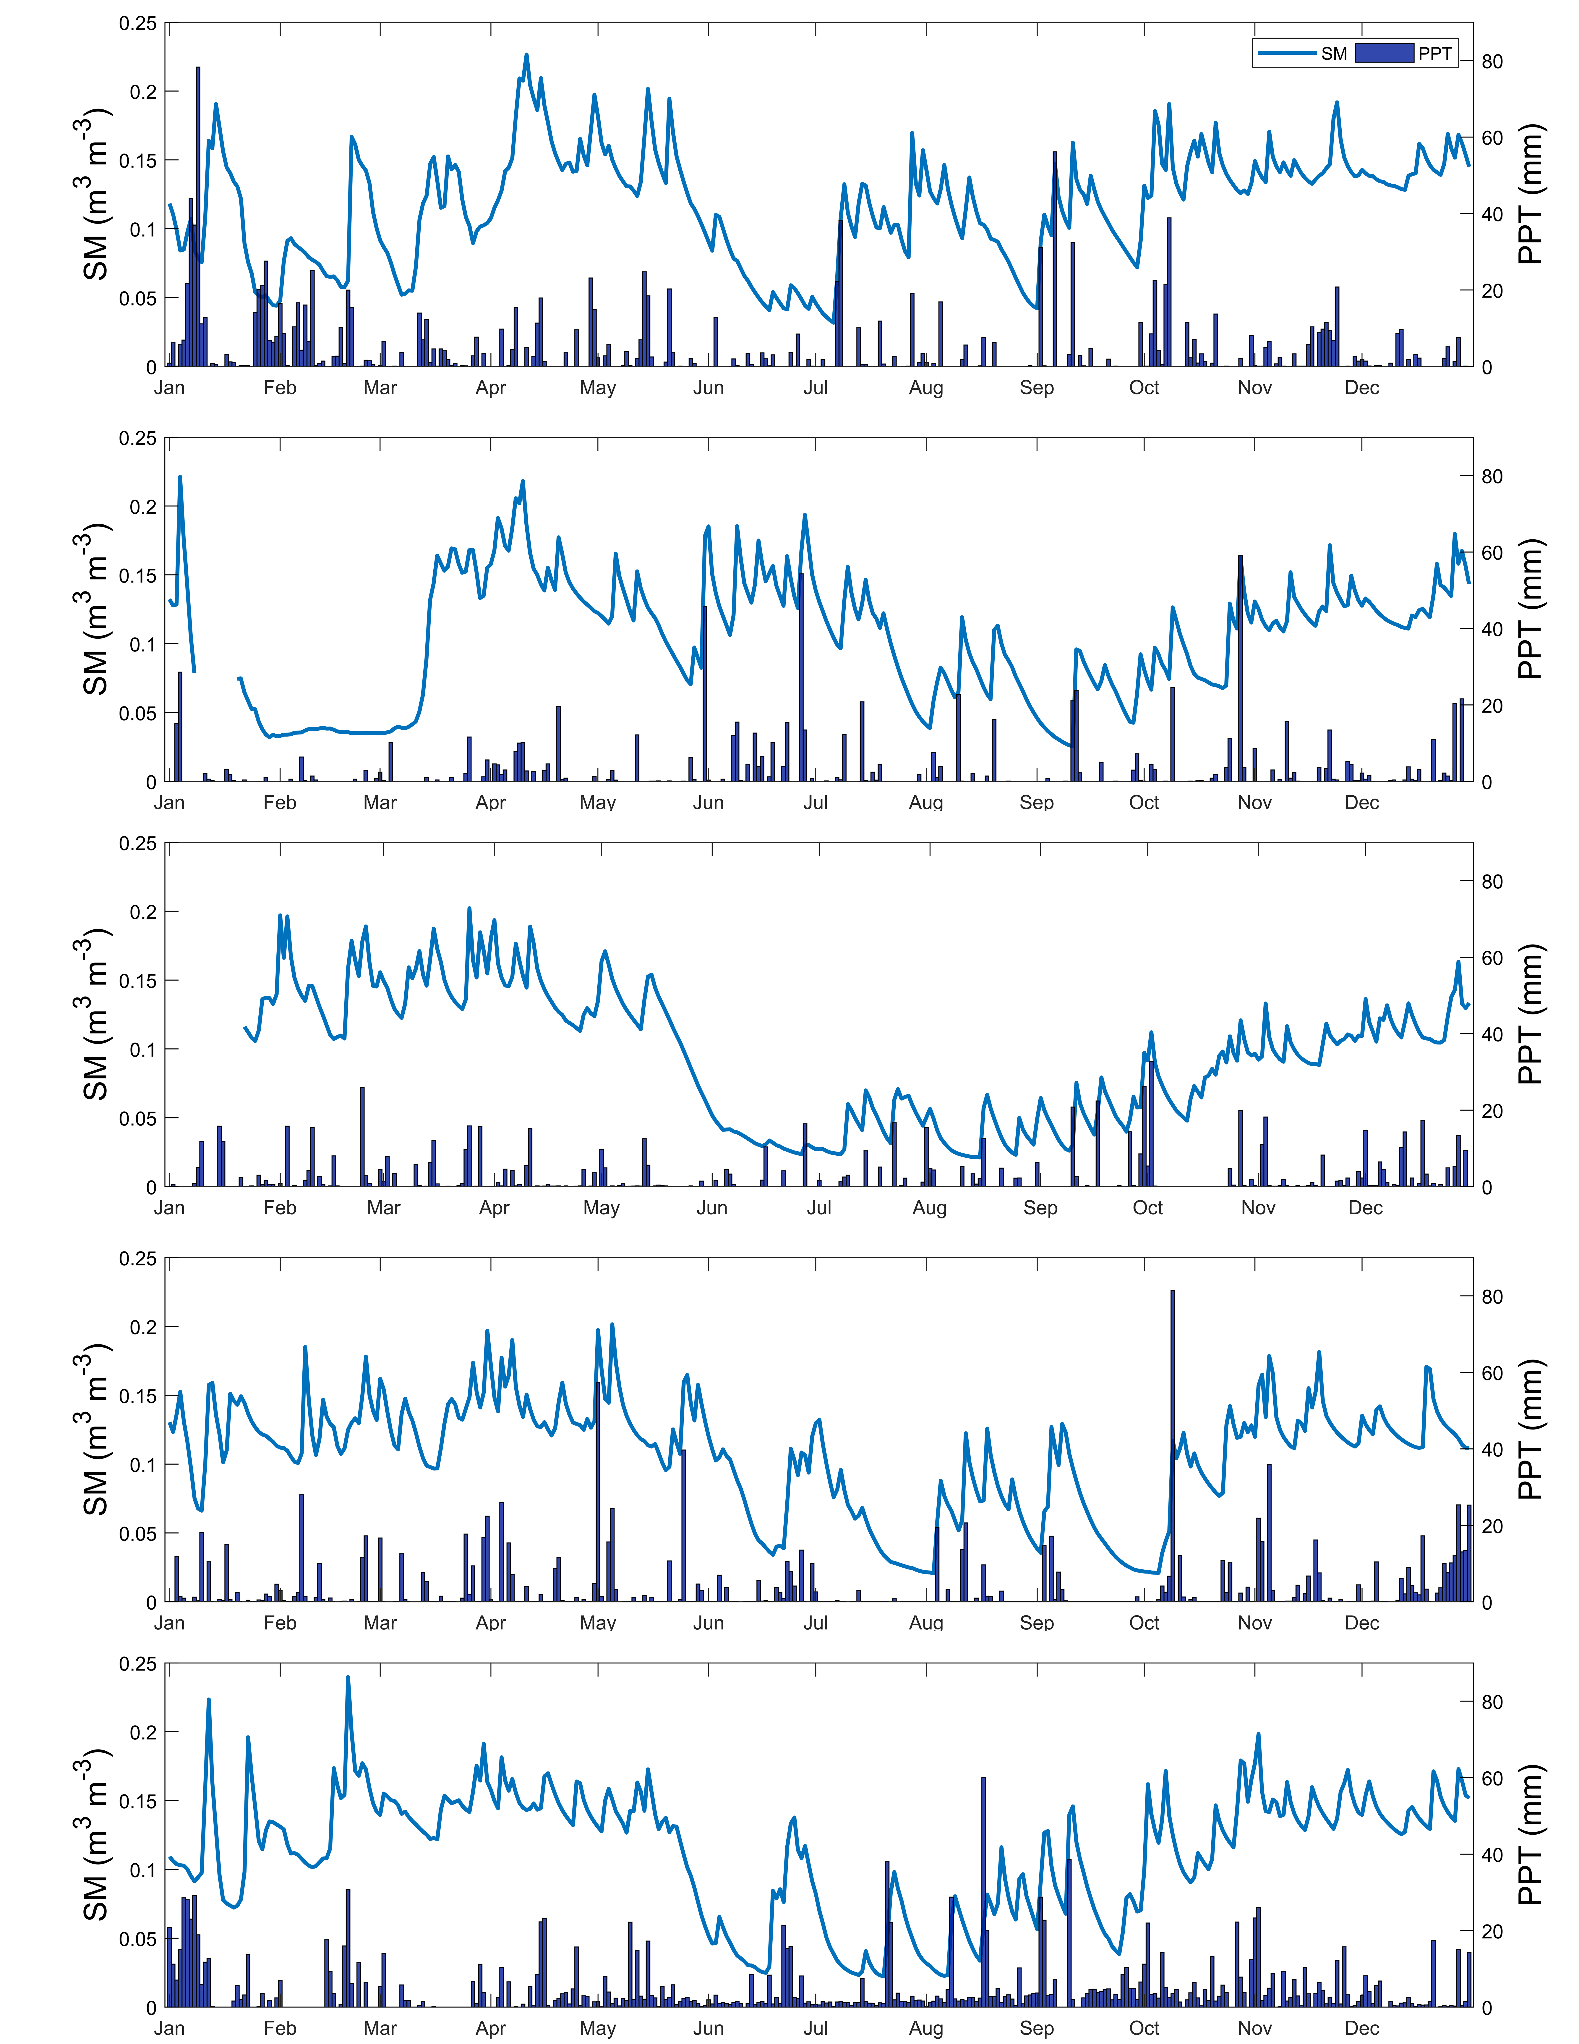
\includegraphics{../images/static/smPPT.png}
\caption{Comparison of daily mean soil mositure content (SM) at 5 cm
depth in m\(^3\) m\(^-\)\(^3\) and cumulative daily average
precipitation (PPT) in mm during (a)2014, (b)2015, (c)2016, (d)2017, and
(e)2018 \label{fig:smPPT}}
\end{figure}

\pagebreak

\hypertarget{references}{%
\section*{References}\label{references}}
\addcontentsline{toc}{section}{References}

\hypertarget{refs}{}
\leavevmode\hypertarget{ref-Apps.1996}{}%
Apps, M.J., Price, D.T., 1996. Forest ecosystems, forest management, and
the global carbon cycle, NATO asi series. Series i, global environmental
change. NATO Advanced Research Workshop The Role of Global Forest
Ecosystems and Forest Resource Management in the Global Cycle; Springer,
Berlin; New York.

\leavevmode\hypertarget{ref-Curielyuste.2004}{}%
Curiel yuste, J., Janssens, I.A., Carrara, A., Ceulemans, R., 2004.
Annual q10 of soil respiration reflects plant phenological patterns as
well as temperature sensitivity. Global Change Biology 10, 161--169.
doi:\href{https://doi.org/10.1111/j.1529-8817.2003.00727.x}{10.1111/j.1529-8817.2003.00727.x}

\leavevmode\hypertarget{ref-Davidson.2006}{}%
Davidson, E.A., Janssens, I.A., 2006. Temperature sensitivity of soil
carbon decomposition and feedbacks to climate change. Nature 440,
165--173.
doi:\href{https://doi.org/10.1038/nature04514}{10.1038/nature04514}

\leavevmode\hypertarget{ref-Edenhofer.2014}{}%
Edenhofer, O. (Ed.), 2014. Climate change 2014: Mitigation of climate
change working group iii contribution to the fifth assessment report of
the intergovernmental panel on climate change. Cambridge University
Press, New York NY.

\leavevmode\hypertarget{ref-GaumontGuay.2006}{}%
Gaumont-Guay, D., Black, T.A., Griffis, T.J., Barr, A.G., Jassal, R.S.,
Nesic, Z., 2006. Interpreting the dependence of soil respiration on soil
temperature and water content in a boreal aspen stand. Agricultural and
Forest Meteorology 140, 220--235.
doi:\href{https://doi.org/10.1016/j.agrformet.2006.08.003}{10.1016/j.agrformet.2006.08.003}

\leavevmode\hypertarget{ref-Greco.1996}{}%
Greco, S., Baldocchi, D.D., 1996. Seasonal variations of co2 and water
vapour exchange rates over a temperate deciduous forest. Global Change
Biology 2, 183--197.
doi:\href{https://doi.org/10.1111/j.1365-2486.1996.tb00071.x}{10.1111/j.1365-2486.1996.tb00071.x}

\leavevmode\hypertarget{ref-Hoff.1899}{}%
Hoff, J.H.v., Lehfeldt, R.A., 1899. Lectures on theoretical and physical
chemistry. E. Arnold, London.

\leavevmode\hypertarget{ref-Jia.2013}{}%
Jia, X., Zha, T., Wu, B., Zhang, Y., Chen, W., Wang, X., Yu, H., He, G.,
2013. Temperature response of soil respiration in a chinese pine
plantation: Hysteresis and seasonal vs. Diel q10. PloS one 8, e57858.
doi:\href{https://doi.org/10.1371/journal.pone.0057858}{10.1371/journal.pone.0057858}

\leavevmode\hypertarget{ref-Khomik.2010}{}%
Khomik, M., Arain, M.A., Brodeur, J.J., Peichl, M., Restrepo-Coupé, N.,
McLaren, J.D., 2010. Relative contributions of soil, foliar, and woody
tissue respiration to total ecosystem respiration in four pine forests
of different ages. Journal of Geophysical Research 115, 237.
doi:\href{https://doi.org/10.1029/2009JG001089}{10.1029/2009JG001089}

\leavevmode\hypertarget{ref-Lee.2002}{}%
Lee, M.-S., Nakane, K., Nakatsubo, T., Mo, W.-h., Koizumi, H., 2002.
Effects of rainfall events on soil co2 flux in a cool temperate
deciduous broad-leaved forest. Ecological Research 17, 401--409.
doi:\href{https://doi.org/10.1046/j.1440-1703.2002.00498.x}{10.1046/j.1440-1703.2002.00498.x}

\leavevmode\hypertarget{ref-Liu2.2016}{}%
Liu, B., Mou, C., Yan, G., Xu, L., Jiang, S., Xing, Y., Han, S., Yu, J.,
Wang, Q., 2016. Annual soil co2 efflux in a cold temperate forest in
northeastern china: Effects of winter snowpack and artificial nitrogen
deposition. Scientific reports 6, 18957.
doi:\href{https://doi.org/10.1038/srep18957}{10.1038/srep18957}

\leavevmode\hypertarget{ref-Liu.2016}{}%
Liu, L., Wang, X., Lajeunesse, M.J., Miao, G., Piao, S., Wan, S., Wu,
Y., Wang, Z., Yang, S., Li, P., Deng, M., 2016. A cross-biome synthesis
of soil respiration and its determinants under simulated precipitation
changes. Global change biology 22, 1394--1405.
doi:\href{https://doi.org/10.1111/gcb.13156}{10.1111/gcb.13156}

\leavevmode\hypertarget{ref-Lorenz.2010}{}%
Lorenz, K., Lal, R., 2010. Carbon sequestration in forest ecosystems.
Springer Netherlands, Dordrecht.

\leavevmode\hypertarget{ref-Matsumoto.2008}{}%
Matsumoto, K., Ohta, T., Nakai, T., Kuwada, T., Daikoku, K., Iida, S.,
Yabuki, H., Kononov, A.V., van der Molen, M.K., Kodama, Y., Maximov,
T.C., Dolman, A.J., Hattori, S., 2008. Energy consumption and
evapotranspiration at several boreal and temperate forests in the far
east. Agricultural and Forest Meteorology 148, 1978--1989.
doi:\href{https://doi.org/10.1016/j.agrformet.2008.09.008}{10.1016/j.agrformet.2008.09.008}

\leavevmode\hypertarget{ref-Mo.2005}{}%
Mo, W., Lee, M.-S., Uchida, M., Inatomi, M., Saigusa, N., Mariko, S.,
Koizumi, H., 2005. Seasonal and annual variations in soil respiration in
a cool-temperate deciduous broad-leaved forest in japan. Agricultural
and Forest Meteorology 134, 81--94.
doi:\href{https://doi.org/10.1016/j.agrformet.2005.08.015}{10.1016/j.agrformet.2005.08.015}

\leavevmode\hypertarget{ref-Pumpanen.2008}{}%
Pumpanen, J., Ilvesniemi, H., Kulmala, L., Siivola, E., Laakso, H.,
Kolari, P., Helenelund, C., Laakso, M., Uusimaa, M., Hari, P., 2008.
Respiration in boreal forest soil as determined from carbon dioxide
concentration profile. Soil Science Society of America Journal 72, 1187.
doi:\href{https://doi.org/10.2136/sssaj2007.0199}{10.2136/sssaj2007.0199}

\leavevmode\hypertarget{ref-Raich.1995}{}%
Raich, J.W., Potter, C.S., 1995. Global patterns of carbon dioxide
emissions from soils. Global Biogeochemical Cycles 9, 23--36.
doi:\href{https://doi.org/10.1029/94GB02723}{10.1029/94GB02723}

\leavevmode\hypertarget{ref-Schlesinger.2000}{}%
Schlesinger, W.H., Andrews, J.A., 2000. Soil respiration and the global
carbon cycle. Biogeochemistry 48, 7--20.
doi:\href{https://doi.org/10.1023/A:1006247623877}{10.1023/A:1006247623877}

\leavevmode\hypertarget{ref-Tang.2014}{}%
Tang, Y., Wen, X., Sun, X., Zhang, X., Wang, H., 2014. The limiting
effect of deep soilwater on evapotranspiration of a subtropical
coniferous plantation subjected to seasonal drought. Advances in
Atmospheric Sciences 31, 385--395.
doi:\href{https://doi.org/10.1007/s00376-013-2321-y}{10.1007/s00376-013-2321-y}

\leavevmode\hypertarget{ref-vanderMolen.2011}{}%
van der Molen, M.K., Dolman, A.J., Ciais, P., Eglin, T., Gobron, N.,
Law, B.E., Meir, P., Peters, W., Phillips, O.L., Reichstein, M., Chen,
T., Dekker, S.C., Doubková, M., Friedl, M.A., Jung, M., van den Hurk,
B.J.J.M., Jeu, R.A.M. de, Kruijt, B., Ohta, T., Rebel, K.T., Plummer,
S., Seneviratne, S.I., Sitch, S., Teuling, A.J., van der Werf, G.R.,
Wang, G., 2011. Drought and ecosystem carbon cycling. Agricultural and
Forest Meteorology 151, 765--773.
doi:\href{https://doi.org/10.1016/j.agrformet.2011.01.018}{10.1016/j.agrformet.2011.01.018}

\leavevmode\hypertarget{ref-Xu.2004}{}%
Xu, L., Baldocchi, D.D., Tang, J., 2004. How soil moisture, rain pulses,
and growth alter the response of ecosystem respiration to temperature.
Global Biogeochemical Cycles 18, n/a--n/a.
doi:\href{https://doi.org/10.1029/2004GB002281}{10.1029/2004GB002281}

\leavevmode\hypertarget{ref-Xu.2001}{}%
Xu, M., Qi, Y., 2001. Soil-surface co2 efflux and its spatial and
temporal variations in a young ponderosa pine plantation in northern
california. Global Change Biology 7, 667--677.
doi:\href{https://doi.org/10.1046/j.1354-1013.2001.00435.x}{10.1046/j.1354-1013.2001.00435.x}

\leavevmode\hypertarget{ref-YiqiLuo.2006}{}%
Yiqi Luo, Xuhui Zhou (Eds.), 2006. Soil respiration and the environment.
Academic Press, Burlington.


\end{document}


